\subsection{Ground Penetrating Radar}

\subsubsection{Fundamentals of Ground Penetrating Radar}

Ground Penetrating Radar (GPR) is a non-invasive subsurface sensing technology that operates by emitting electromagnetic (EM) waves and analyzing their reflections to detect objects embedded underground. A typical GPR system consists of an active sensor and a wideband antenna, which transmits EM waves into the ground and receives the backscattered signals from interfaces where there is a contrast in electrical properties---such as between soil and buried objects. The reflection characteristics---both in direction and intensity---depend on the roughness of the interface and the dielectric properties of the materials involved ~\cite{paik2002image}.

In GPR systems, the presence of a buried object is inferred from discontinuities in the round-trip signal path. The time delay $\Delta t$ between the transmission and reception of a wave is used to calculate the depth of the target via the relation:
\[
R = \frac{v \cdot \Delta t}{2} ~\cite{paik2002image}
\]
where $v$ is the wave velocity in the medium (which varies with soil properties), and $R$ is the estimated distance to the object.

To visualize GPR data, three types of scans are commonly used: \textbf{A-scan}, \textbf{B-scan}, and \textbf{C-scan}. A-scans represent 1D reflections at a single point, showing signal strength versus time delay. B-scans compile a series of A-scans along a line to form a 2D profile of the subsurface, while C-scans aggregate B-scans from multiple parallel lines to generate a volumetric 3D map of the ground. 

Figure~\ref{fig:gpr_coords} illustrates the 3D coordinate system used in GPR scanning, where A-scans are acquired vertically into the ground (z-direction) at multiple $(x', y')$ positions. By scanning along the x-direction, a B-scan is formed, and repeating this across different y-values enables construction of a C-scan. Figure~\ref{fig:gpr_bscan} shows a sample B-scan image acquired at a fixed $y'$ location, where hyperbolic signatures in the time-delay domain represent buried objects~\cite{paik2002image}. 

Since our project focuses on localizing and estimating the depth of landmines, rather than reconstructing their full 3D geometry, we would be collecting B-scan data on the drone.

\begin{figure}[h!]
    \centering
    \begin{subfigure}[b]{0.48\linewidth}
        \centering
        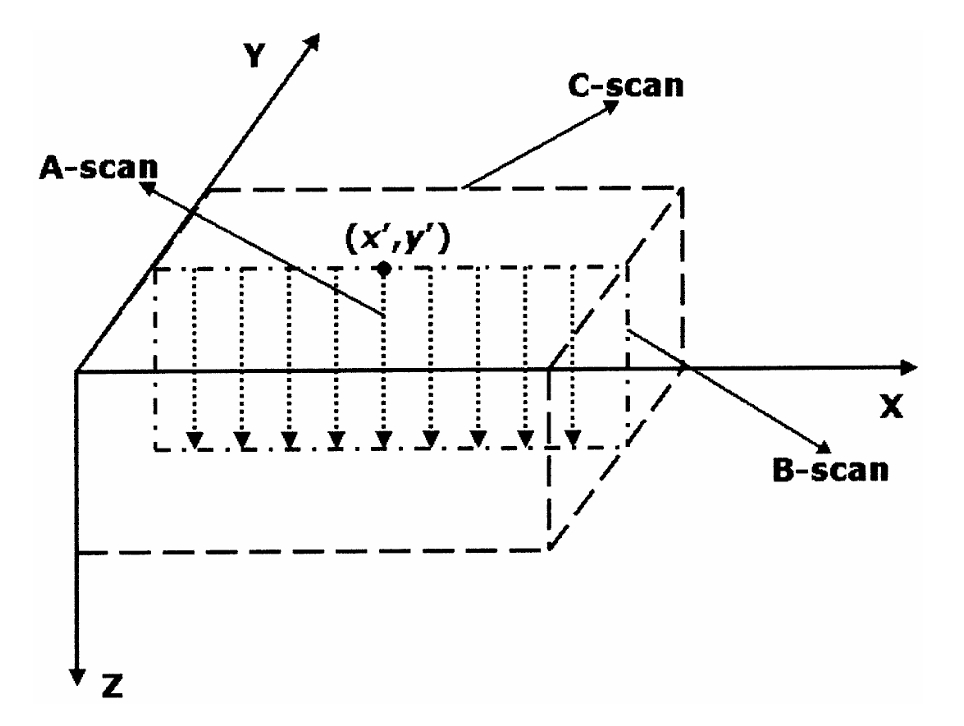
\includegraphics[width=\linewidth]{figs/Huirui/gpr_coords.png}
        \caption{Coordinate convention for GPR scanning.}
        \label{fig:gpr_coords}
    \end{subfigure}
    \hfill
    \begin{subfigure}[b]{0.48\linewidth}
        \centering
        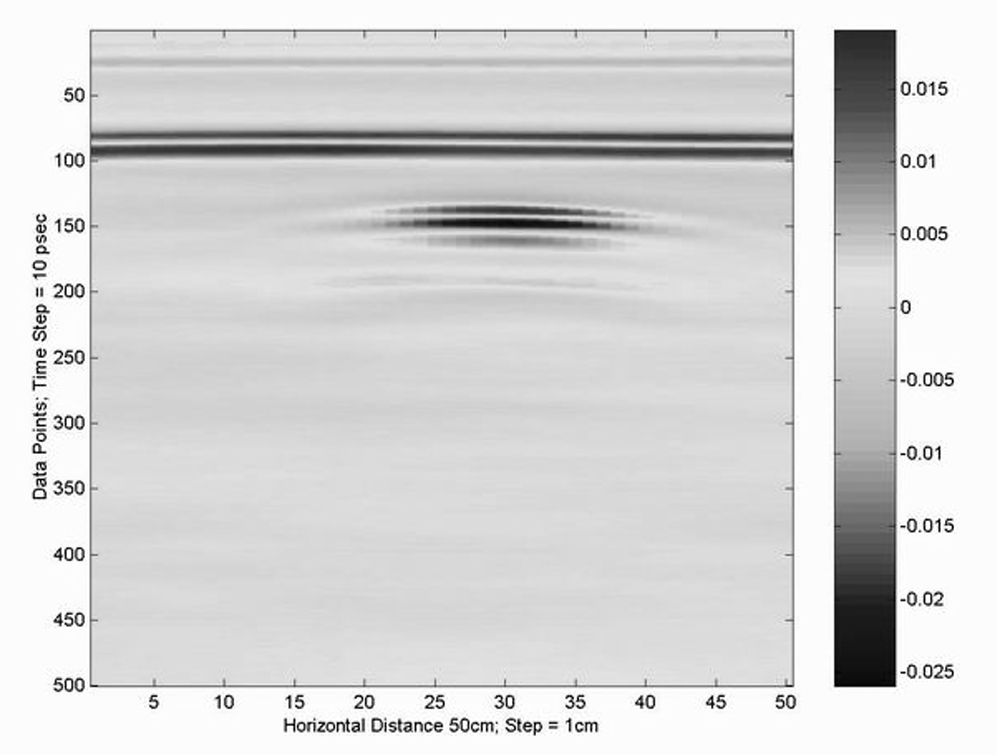
\includegraphics[width=\linewidth]{figs/Huirui/gpr_bscan.png}
        \caption{Example of a B-scan.}
        \label{fig:gpr_bscan}
    \end{subfigure}
    \caption{Visualization of GPR data acquisition and interpretation~\cite{paik2002image}.}
\end{figure}


\subsubsection{Design Factors Influencing GPR Performance}

The effectiveness of a Ground Penetrating Radar (GPR) system for UAV-based landmine detection depends on a variety of factors that influence its resolution, penetration depth, system complexity, and integration feasibility. These include waveform generation mechanisms, signal frequency characteristics, resolution metrics, antenna design, advanced signal processing techniques such as Synthetic Aperture Radar (SAR), and overall system orientation with respect to the ground. This section introduces the key considerations that inform GPR design and their impact on airborne applications.

\paragraph{Waveform Type}

The waveform type determines how the radar transmits and receives electromagnetic signals. The three most common waveform types used in GPR are summarized below:

\begin{itemize}
    \item \textit{Impulse (pulsed) GPR}: it transmits ultra-short pulses with broad spectral content, enabling ultra-wideband (UWB) operation and high-resolution imaging. These systems are simple and low-cost but require high-speed ADCs or subsampling receivers to handle the wide instantaneous bandwidth~\cite{chen2023ground,sipos2017drone}.
    \item \textit{Frequency-Modulated Continuous Wave (FMCW) GPR}: it transmits a chirp signal with a frequency that increases over time. It offers better average transmitted power and potentially improved signal-to-noise ratio but is hardware-intensive and more susceptible to phase noise and motion errors~\cite{burr2018design}.
    \item \textit{Stepped-Frequency Continuous Wave (SFCW) GPR}: it steps through discrete frequencies and collects reflections in the frequency domain. The collected data are transformed back into the time domain using an inverse Fourier transform. While offering high signal-to-noise ratio and reduced ADC requirements, SFCW systems often perform poorly in air-launched UAV applications due to limited ground coupling and dominant surface reflections~\cite{tronca2018comparison}.
\end{itemize}


\paragraph{Center Frequency, Bandwidth, Resolution, and Penetration Depth}

The radar signal’s center frequency and bandwidth jointly determine the GPR system’s ability to resolve targets and penetrate subsurface layers. Lower frequencies (e.g., < 1 GHz) enhance penetration depth but limit resolution. Higher frequencies (e.g., > 2--3 GHz) improve resolution but attenuate quickly, especially in moist or conductive soils. For instance, a GPR operating at 3 GHz may penetrate up to 0.5 m in dry soil, but only a few centimeters in wet soil~\cite{alqudsi2021review}. This trade-off is illustrated in Figure~\ref{fig:freq_tradeoff}, where increasing frequency leads to improved resolution but reduced sensing depth.

\begin{figure}[h!]
    \centering
    \begin{subfigure}[b]{0.48\linewidth}
        \centering
        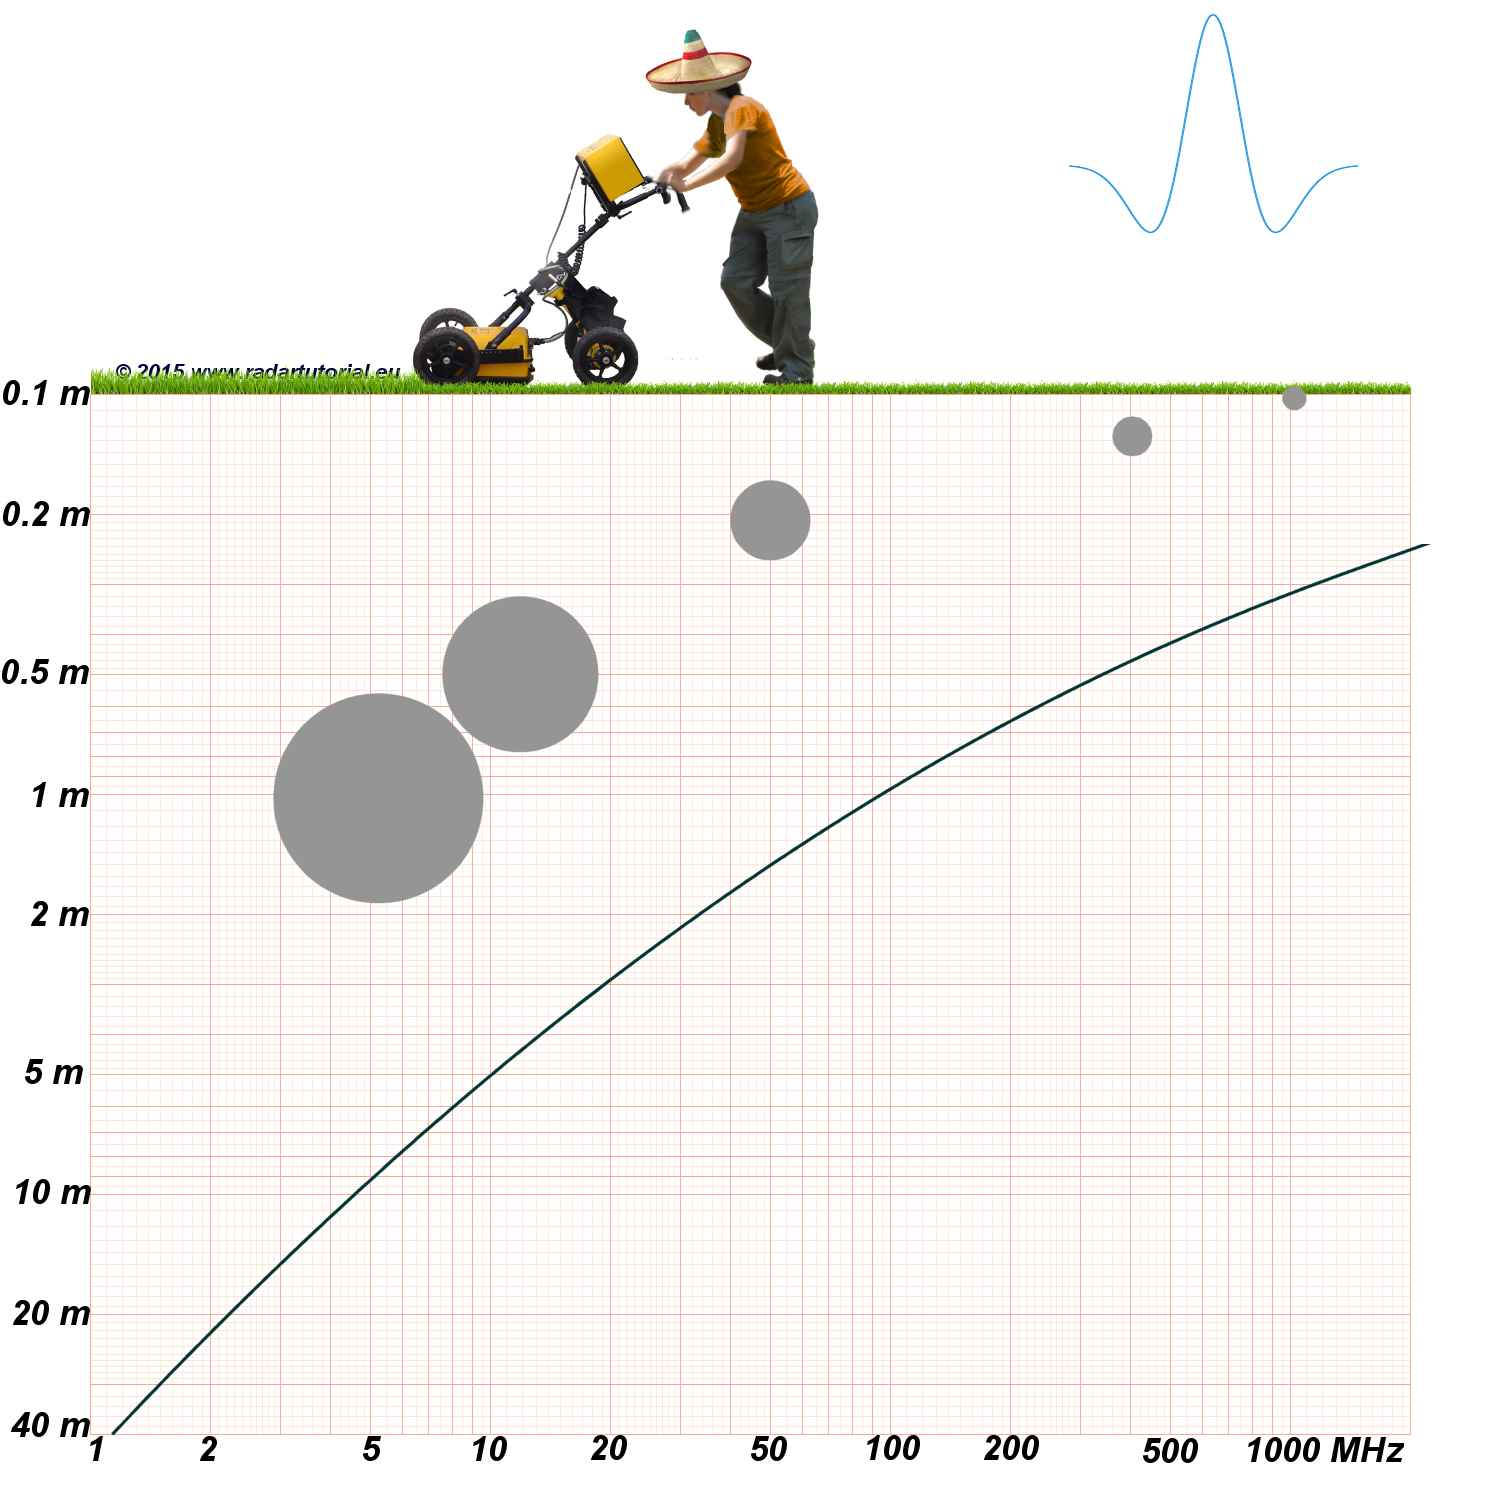
\includegraphics[height=4cm]{figs/Huirui/freq_tradeoff.png}
        \caption{Frequency–resolution vs. penetration depth trade-off\protect\footnotemark.}
        \label{fig:freq_tradeoff}
    \end{subfigure}
    \hfill
    \begin{subfigure}[b]{0.48\linewidth}
        \centering
        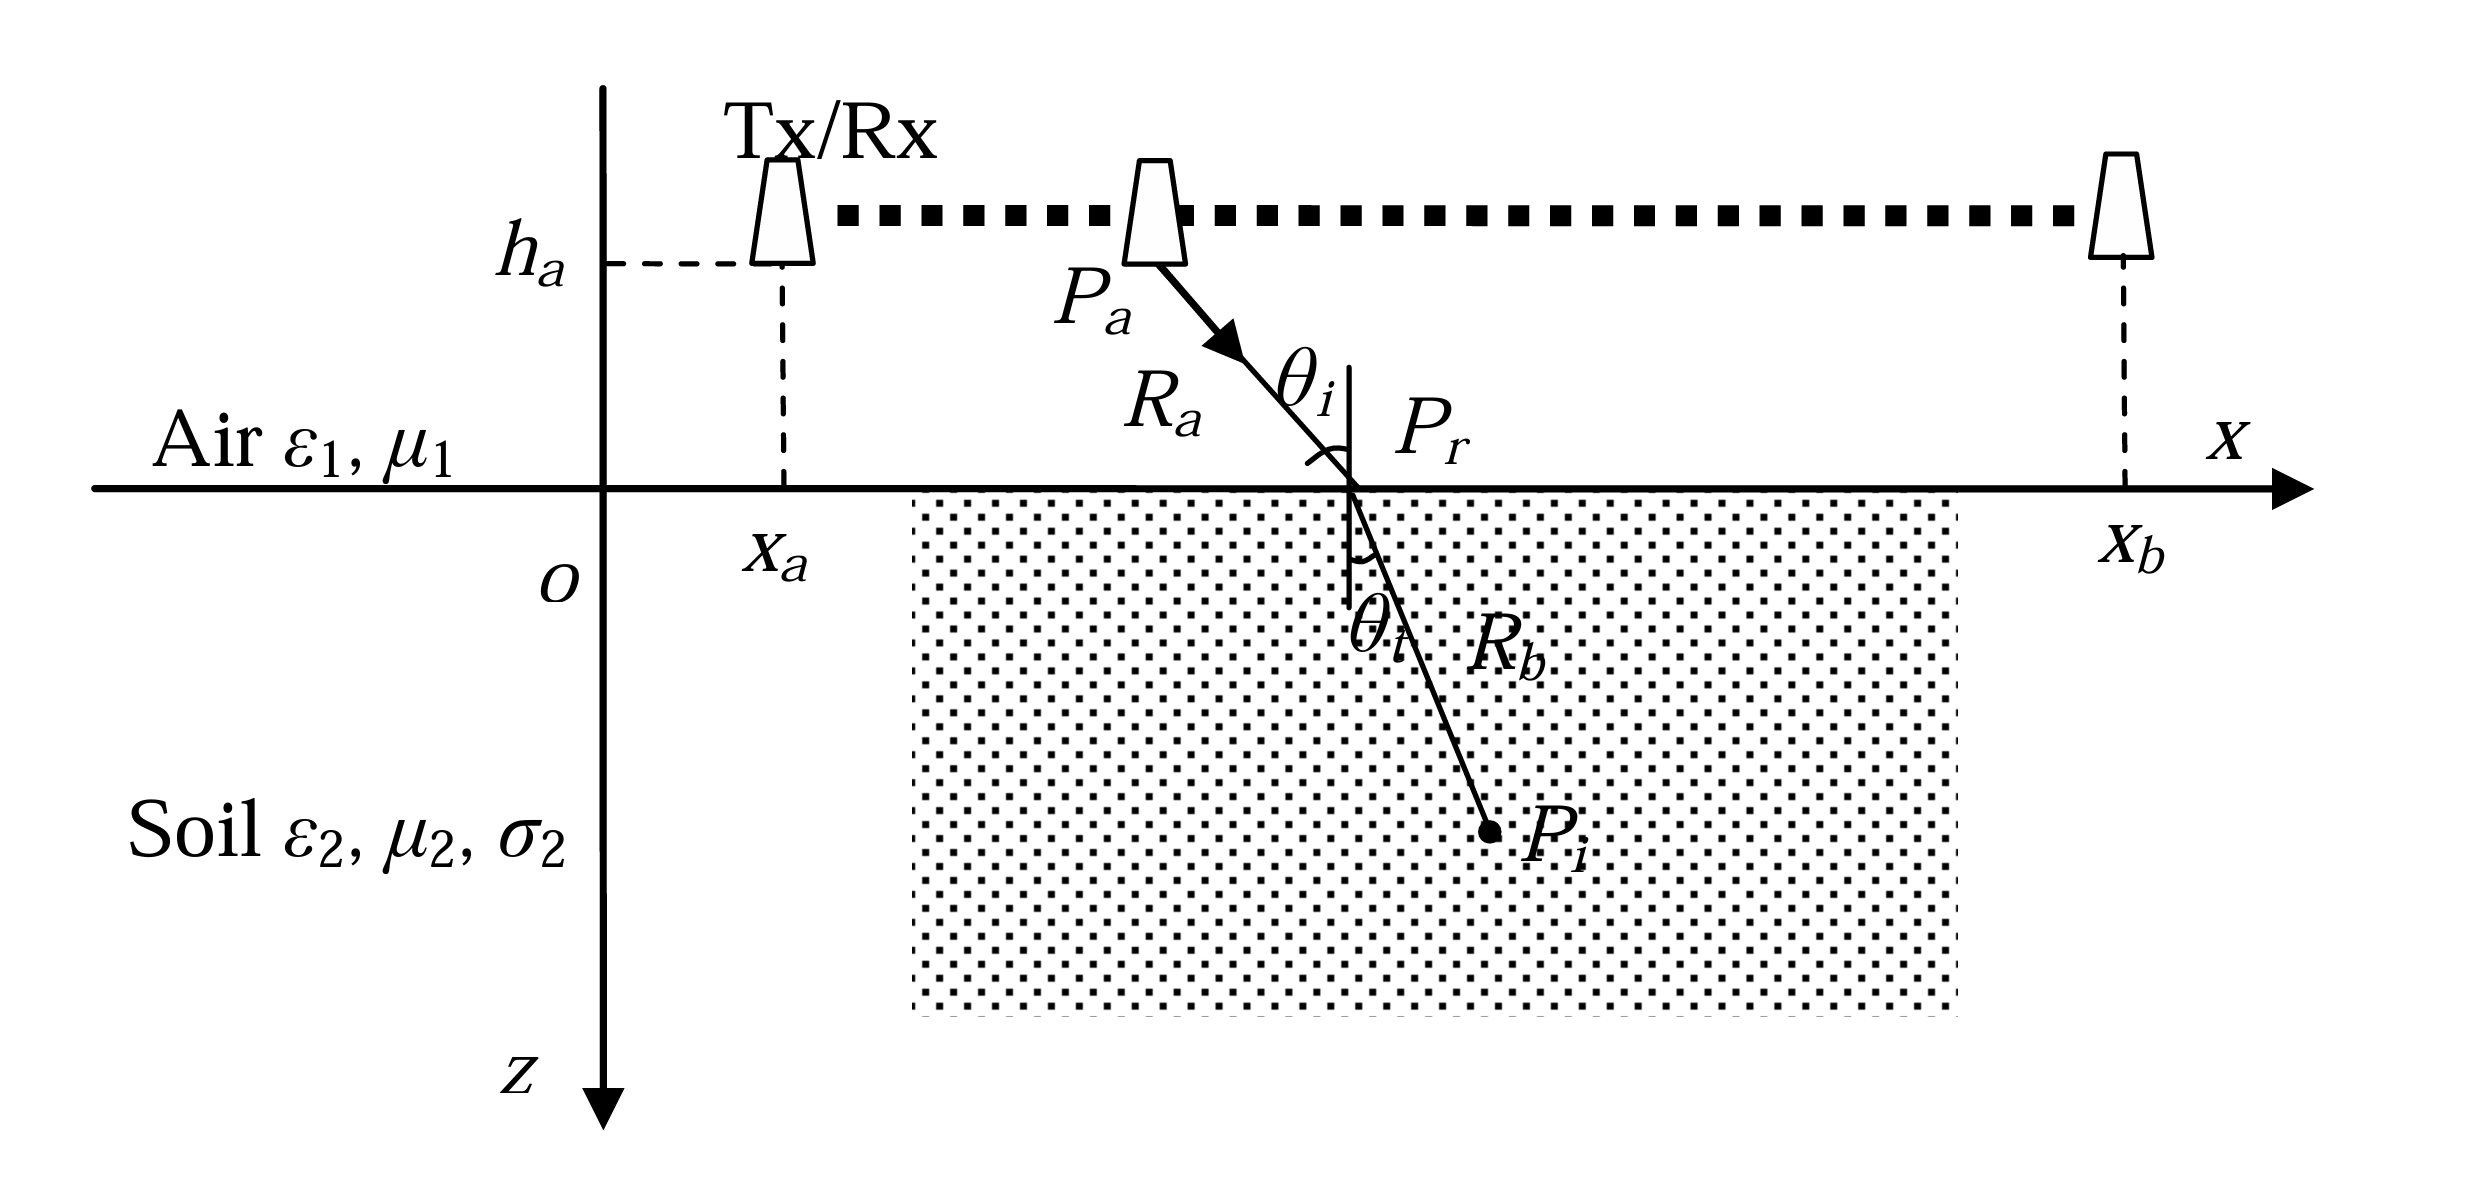
\includegraphics[height=4cm]{figs/Huirui/bp_geometry.png}
        \caption{Illustration of BP imaging geometry~\cite{lei2014multi}.}
        \label{fig:bp_geometry}
    \end{subfigure}
\end{figure}


Bandwidth, defined as the difference between the maximum and minimum frequencies $B = f_{\text{max}} - f_{\text{min}}$, governs the radar’s range (or depth) resolution $\Delta r$, which is the ability to differentiate between objects located at different depths along the same vertical axis. Under free-space conditions, where the wave velocity $v_p = c$ (the speed of light), the range resolution $\Delta r$ is approximated by:
\[
\Delta r = \frac{c}{2B}~\cite{alqudsi2021review}
\]
where $c$ is the speed of light in vacuum.

\footnotetext{\url{www.radartutorial.eu}}


Cross-range or lateral resolution $\Delta l$ describes the radar’s ability to distinguish objects side by side at the same depth. It depends on the central wavelength $\lambda_c$ and aperture size $L_{\text{ap}}$, and in free-space is approximated by:
\[
\Delta l = \frac{R \lambda_c}{L_{\text{ap}}}~\cite{alqudsi2021review}
\]
with $R$ as the antenna-to-target distance.


\paragraph{Synthetic Aperture Radar (SAR) Processing}

Traditional GPR systems suffer from limited cross-range resolution due to the physical constraints of the antenna aperture. SAR overcomes this limitation by coherently integrating radar echoes collected along the UAV’s flight path, effectively synthesizing a much larger aperture. This enables fine lateral resolution imaging using small, lightweight antennas — a critical benefit for UAV-mounted GPR systems~\cite{alqudsi2021review}.

Among SAR methods, \textit{Back-Projection (BP)} is particularly suited to UAV-based GPR due to its flexibility in handling irregular flight trajectories and non-uniform measurement spacing. It works by summing radar echoes along computed time-delay curves for each focal point in the subsurface. As illustrated in Figure~\ref{fig:bp_geometry}, the UAV-mounted radar collects signals $e_1(x_p, t)$ at positions $x_p$ along the flight path. The round-trip travel time $\tau_{m,n,p}$ from the transmitter to a target point $(x_n, z_m)$ and back is used to time-shift and coherently sum these signals:
\[
e_2(x_n, z_m) = \sum_{p=1}^{P} e_1(x_p, \tau_{m,n,p})~\cite{lei2014multi}
\]
\[
\tau_{m,n,p} = \frac{2R_a}{c} + \frac{2R_b}{v}~\cite{lei2014multi}
\]
where $R_a$ and $R_b$ are the distances in air and in soil, respectively, $c$ is the speed of light in air, and $v$ is the wave velocity in the soil medium. This delay-and-sum approach transforms hyperbolic reflections in conventional B-scans into focused point targets, improving interpretability. However, it is computationally expensive and thus not well-suited for real-time onboard processing~\cite{lei2014multi}.

SAR systems can operate in several modes depending on how the radar beam is managed during flight, as shown in Figure~\ref{fig:sar_modes}:

\begin{itemize}
    \item \textbf{Stripmap SAR}: The radar beam remains fixed relative to the UAV, illuminating a continuous swath as the platform moves forward. It provides a good balance between coverage area and azimuth resolution~\cite{moreira2013tutorial}.
    \item \textbf{ScanSAR}: The beam is periodically steered across multiple sub-swaths, expanding coverage at the cost of degraded resolution~\cite{moreira2013tutorial}.
    \item \textbf{Spotlight SAR}: The beam is focused on a single point for an extended time to maximize resolution, but at the expense of imaging area~\cite{moreira2013tutorial}.
\end{itemize}


\paragraph{GPR Sensor Orientation}

The orientation of a UAV-mounted GPR system significantly affects its imaging performance and integration feasibility. Below are the two types of radar orientions, as shown in Figure~\ref{fig:GPR_Ori_modes}:

\begin{itemize}
    \item \textbf{Forward-Looking (FLGPR) or Side-Looking} directs radar waves obliquely into the ground, reducing surface clutter but receiving only weak backscatter from buried targets. It requires high dynamic range receivers and is typically better for shallow target detection~\cite{garcia2020airborne}.
    \item \textbf{Down-Looking (DLGPR)} points antennas perpendicularly toward the ground, maximizing reflected signal strength from targets but introducing stronger surface clutter~\cite{garcia2020airborne}.
\end{itemize}


\begin{figure}[h!]
    \centering
    \begin{subfigure}[b]{0.48\linewidth}
        \centering
        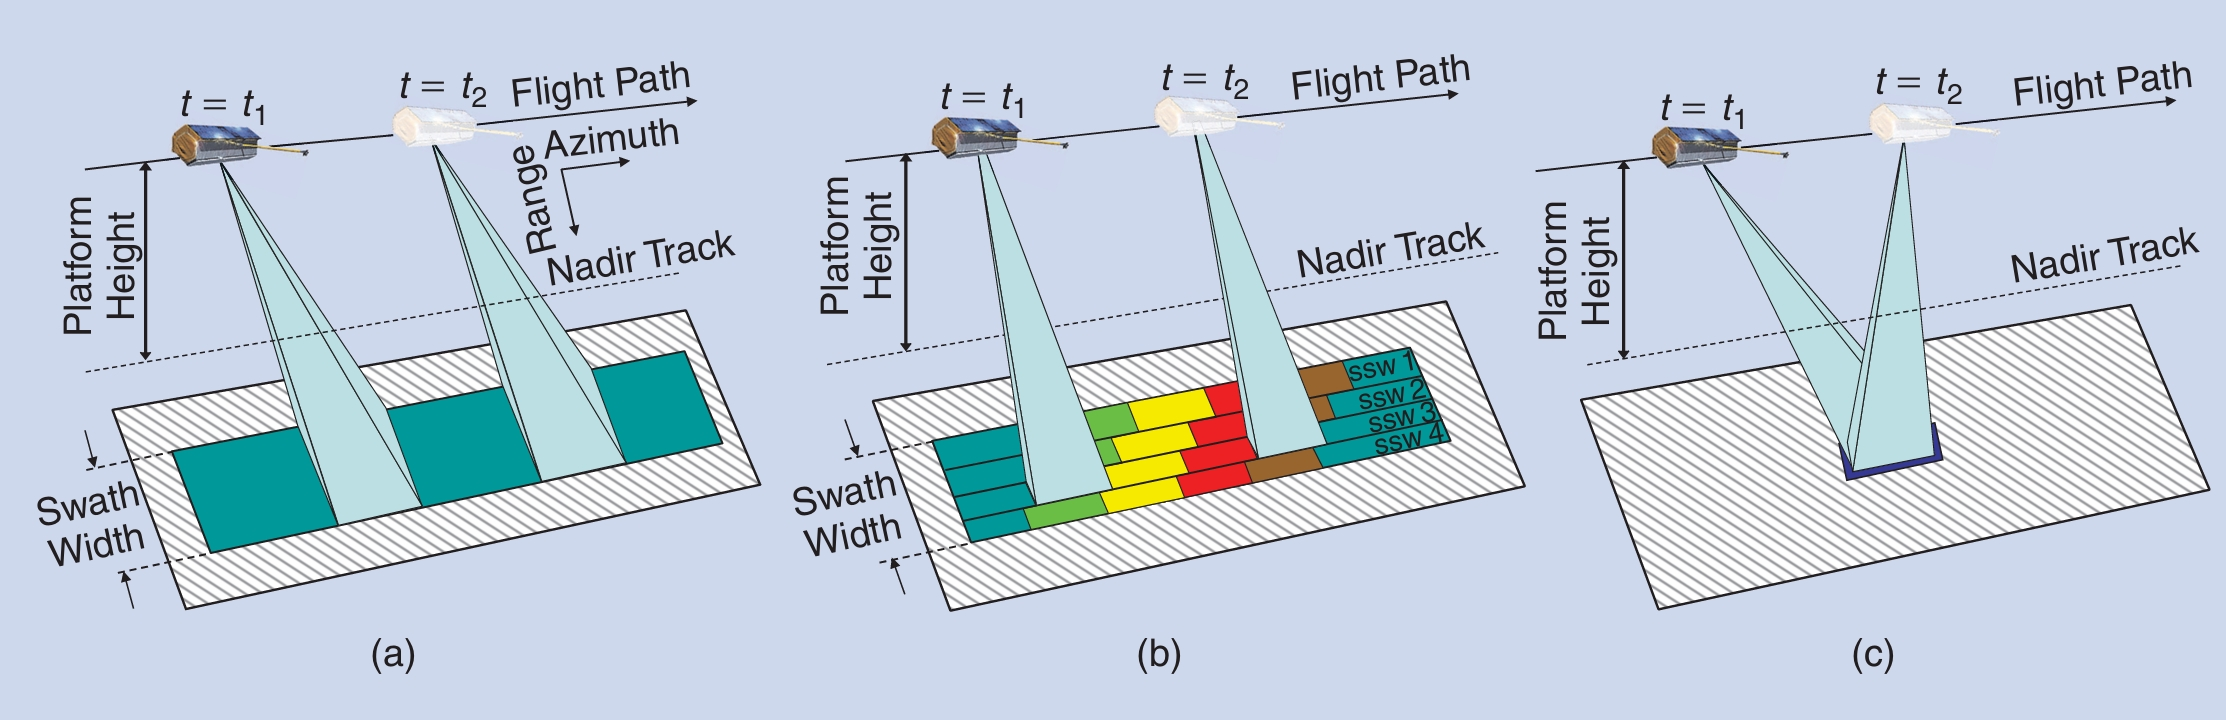
\includegraphics[width=\linewidth]{figs/Huirui/sar_modes.png}
        \caption{Illustration of different SAR operation modes~\cite{moreira2013tutorial}.}
        \label{fig:freq_tradeoff}
    \end{subfigure}
    \hfill
    \begin{subfigure}[b]{0.48\linewidth}
        \centering
        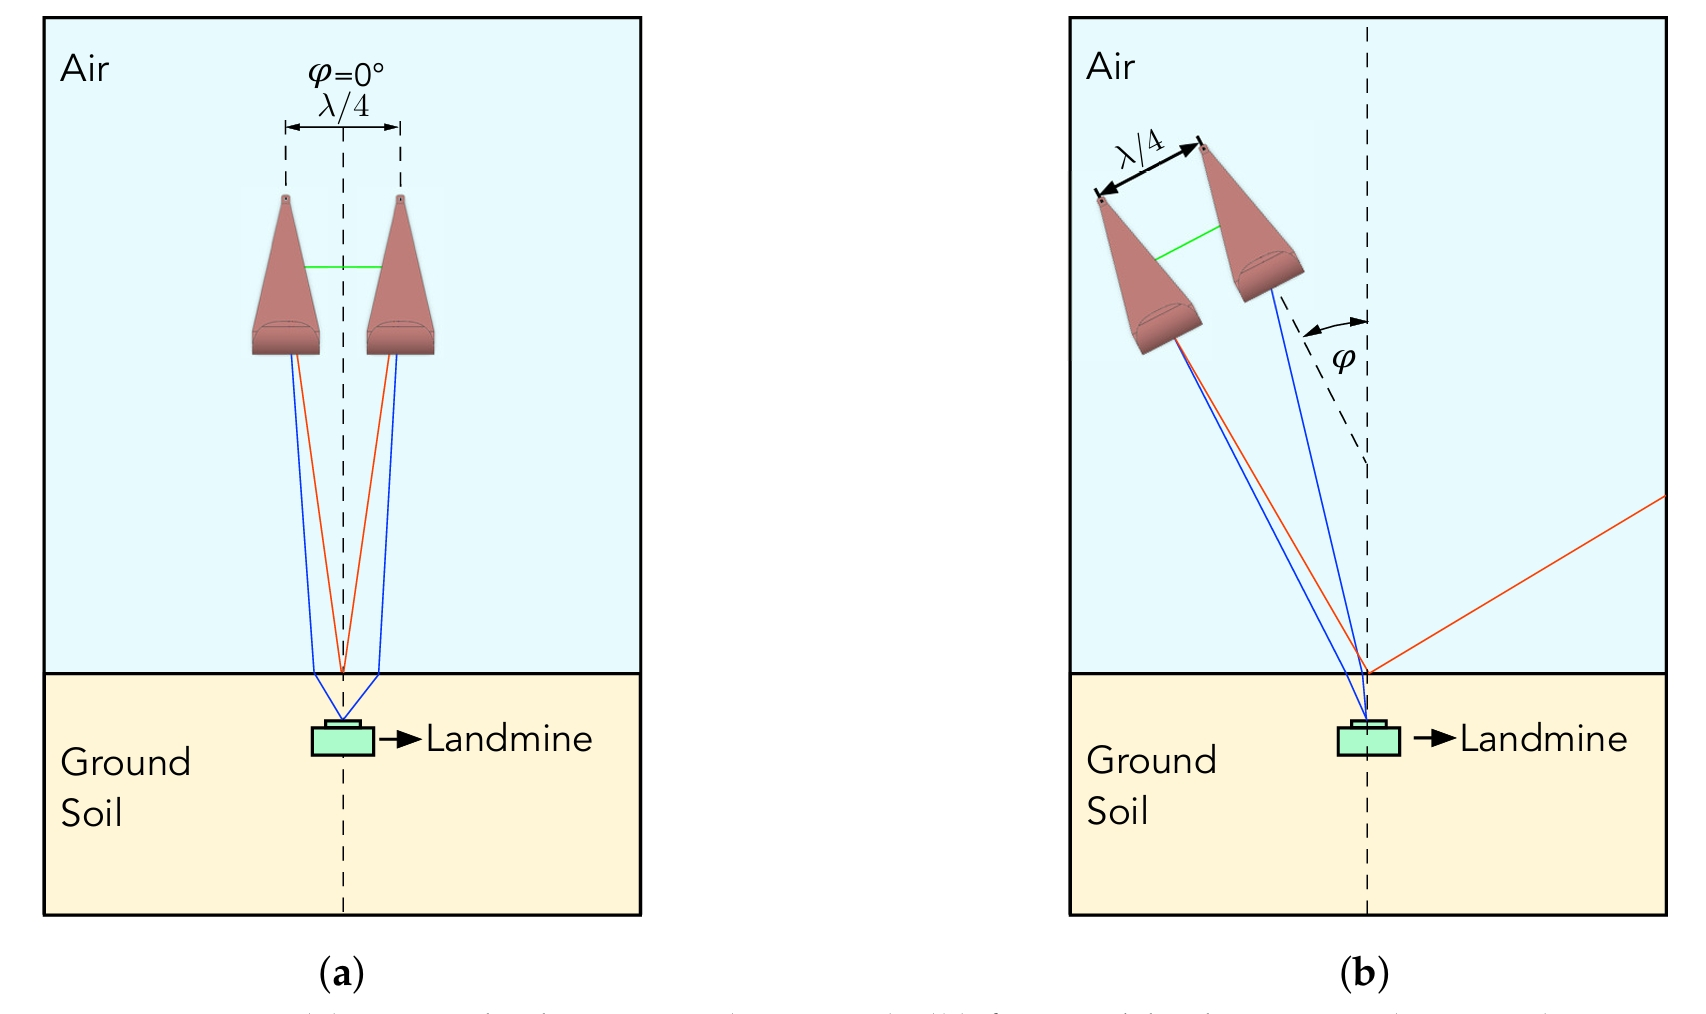
\includegraphics[width=\linewidth]{figs/Huirui/gpr_ori_modes.png}
        \caption{(a) DLGPR; (b) FLGPR~\cite{vsipovs2020lightweight}.}
        \label{fig:bp_geometry}
    \end{subfigure}
\end{figure}


\paragraph{Antenna Size and Type}

Antenna size is inversely related to frequency, and a rough estimate for the required physical length is:
\[
L_{\text{antenna}} \approx \frac{\lambda_{\text{min}}}{2}
\]
where  $\lambda_{\text{min}}$ is the wavelength of the minimum GPR frequency.

This imposes a trade-off between desired penetration (favoring low frequencies) and UAV payload constraints (favoring compact antennas)~\cite{alqudsi2021review}.


These factors collectively inform the design trade-offs necessary to build an effective UAV-compatible GPR system. Our final choices based on these considerations are summarized and justified in the following subsection.


\subsubsection{System Configuration and Design Rationale}

While a wide range of GPR architectures have been explored in past research, most high-performance UAV-based landmine detection systems rely on custom-designed radar platforms to maximize resolution, penetration, and real-time adaptability. These advanced systems often use Software-Defined Radio (SDR), custom waveform control, and specialized antenna arrays to improve their performance for specific soil conditions and mission requirements ~\cite{cerquera2017uav}.

However, the focus of our project is on demonstrating the feasibility of integrating GPR into a multi-UAV architecture for landmine detection in conjunction with high-altitude thermal imaging. Given this goal and the constraints on time, budget, and hardware development, we propose using a commercial off-the-shelf (COTS) impulse GPR unit for the first version of our system.

Specifically, we select the {SPH Engineering Zond Aero 1000 MHz GPR, which is a lightweight (approx.\ 1.8 kg\footnote{\label{Zond}\url{https://cdn.shopify.com/s/files/1/0596/9451/4353/files/RadSys_Zond_Aero_1000_NG_datasheet.pdf?v=1732295405}}) impulse radar designed for UAV integration. It operates in the 600–1300~MHz band with a central frequency of 1 GHz\textsuperscript{\ref{Zond}}, offering a reasonable balance between resolution and subsurface penetration. Compared to high-frequency systems that provide finer resolution but shallow depth, this system emphasizes depth penetration, which is more important than resolution for detecting mines that may be buried in compact or moist soils. While the this system's vertical resolution (around 10--15~cm) may not allow precise depth estimation, this limitation is acceptable for our application, where the primary objective is to confirm the presence of subsurface anomalies rather than reconstruct their exact geometry.

The system uses a DLGPR configuration, which ensures maximum power reflection from subsurface targets and simplifies mounting on the UAV due to its symmetric layout. While DLGPR does introduce surface clutter due to strong air–ground reflections, these can be mitigated through signal processing techniques such as Singular Value Decomposition (SVD) and migration algorithms ~\cite{garcia2024comparison}. Furthermore, DLGPR is the most widely adopted orientation in existing UAV-GPR systems, supporting its practical benefits ~\cite{alqudsi2021review}.

To enhance lateral resolution and mitigate the poor range resolution of low-frequency radar, we implement SAR processing using the Stripmap mode with a BP algorithm. This configuration enables continuous-area scanning without requiring beam steering, which reduces UAV control complexity. BP supports flexible trajectory handling and achieves improved focusing, which is especially beneficial when verifying thermally indicated hotspots. The feasibility of SAR processing in our system is enabled by the centimeter-level positioning accuracy provided by our customized GNSS and IMU module, which ensures precise geo-referencing of each radar acquisition point. Given the computational intensity of the BP algorithm, processing is conducted offline after the flight mission, consistent with our plan to store raw B-scans for post-processing rather than attempt onboard real-time detection.

This system architecture based on a COTS impulse radar with low-frequency operation and offline SAR processing represents a practical and achievable foundation for our project's first implementation. It allows us to demonstrate the viability of UAV-mounted GPR for landmine detection while leaving room for future enhancements such as SDR-based signal control or custom radar front-end development in later project stages.


\subsubsection{Flight Parameters and Sampling Considerations}

In our system, the GPR drone is designed to fly at an altitude of approximately 2 meters. This low-altitude range ensures effective power coupling into the ground while maintaining safe clearance for the UAV during low-level autonomous operations. The selected height aligns with previous studies and implementations using down-looking impulse GPR for landmine detection ~\cite{schartel2018uav,alqudsi2021review}.

Assuming a down-looking antenna configuration with a beamwidth of $\theta = 45^\circ$, the effective swath width $W$ covered by the radar during a single pass can be estimated using the geometric formula:
\[
W = 2h \cdot \tan\left(\frac{\theta}{2}\right)
\]
For $h = 2$ m, the resulted swath width is 1.65 m. This defines the effective width of ground coverage per flight strip. Figure~\ref{fig:swath_geometry} illustrates the geometry, noting that for our DLGPR, the radar angle $\alpha$ is set to $90^\circ$.

\begin{figure}[H]
    \centering
    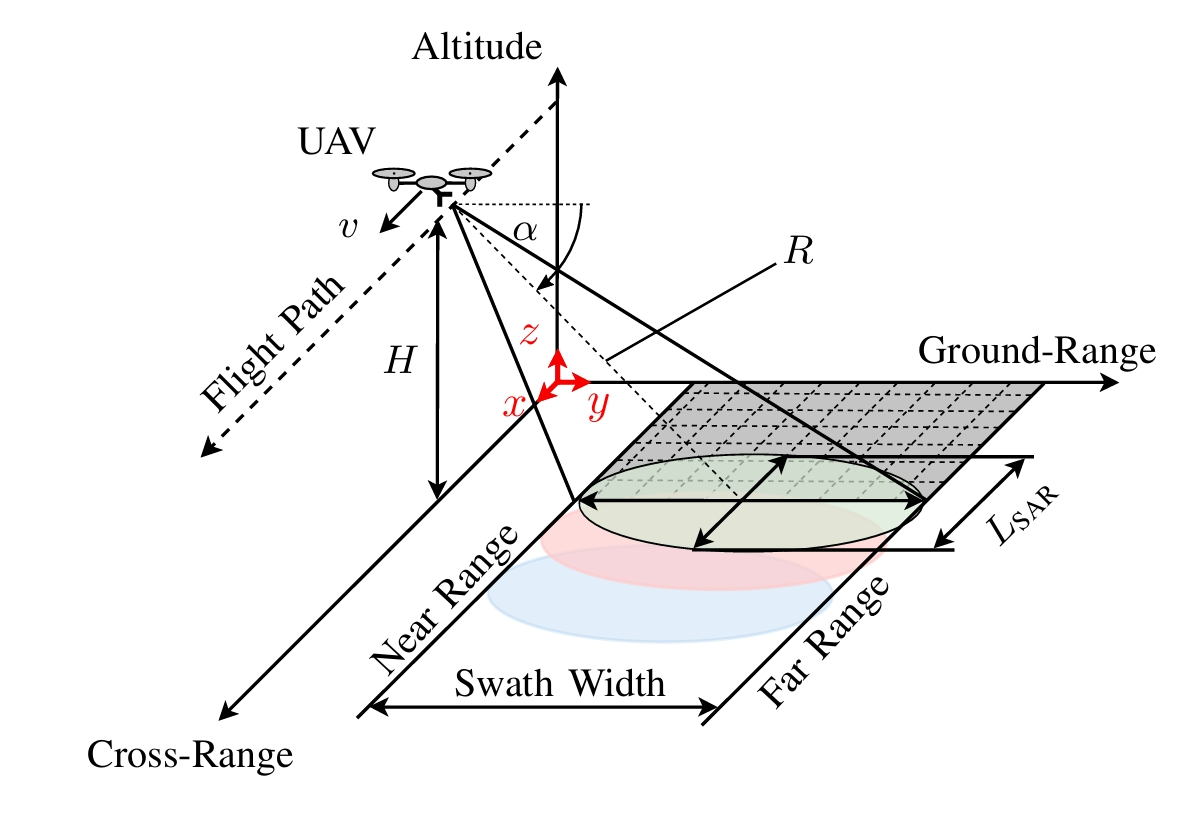
\includegraphics[width=0.6\textwidth]{figs/Huirui/gpr_swath}
    \caption{Illustration of the stripmap SAR geometry.~\cite{schartel2018uav}.}
    \label{fig:swath_geometry}
\end{figure}

To support SAR image reconstruction using the BP algorithm, the radar measurements must satisfy the Nyquist spatial sampling criterion. This condition ensures that the maximum spacing $\Delta x$ between successive acquisition points does not exceed half the wavelength corresponding to the maximum radar frequency:
\[
\Delta x \leq \frac{\lambda_{\text{min}}}{2}
\]
For our system, the maximum operating frequency is 1.3 GHz, the maximum allowable sampling interval is 11.5 cm. Given the estimated thermal camera coverage of 9 m × 7 m, with a zig-zag flight path, a total of 332 acquisition points for one thermal-indicated area need to be visited. 